\chapter{Mission Planning}
  \paragraph{
  		Even when flying as a wingman, each pilot should do his best to prepare for the flight. In a training scenario it is important to train as many aspects of flying as possible, and during a combat mission the wingman might find himself in a position where he has to act as lead. It is therefore important to understand and practice acquiring the relevant information to your flight. It is equally important to perform a debrief and submit your after-action report after the flight is completed. \\
  }
  
\section{Frequencies}
  \textnormal{
  	For the purpose of communication, the 132nd utilizes a frequency table containing all frequencies currently employable by the wing. The left column has a codeword (color), and the top rows has a number. Together they form a codeword for each frequency. The reason for this is to avoid transmitting operational frequencies on open, unencrypted radio. Figure \ref{opfreqs} shows the current table as of January 2018. \\
  }
  
  \textnormal{
  	The Mirage 2000C is equipped with two programmable radios. By default, these are programmed to the frequencies shown in figure \ref{presets} unless otherwise stated. The exception might be some combat missions and campaigns, and if we are flying on other servers. \\
  }
  
  \begin{figure}[!ht]
  	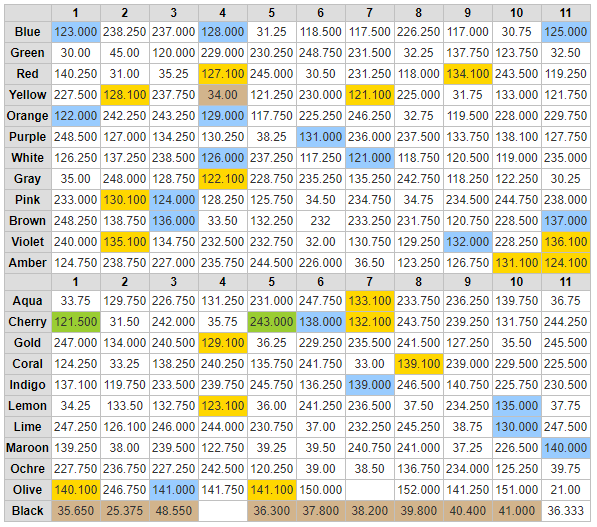
\includegraphics[scale=0.9]{frequencies.png}
    	\label{opfreqs}
    	\caption{List of 132nd Operational Frequencies as of January, 2018}
  \end{figure}
  
  \begin{figure}[!ht]
  	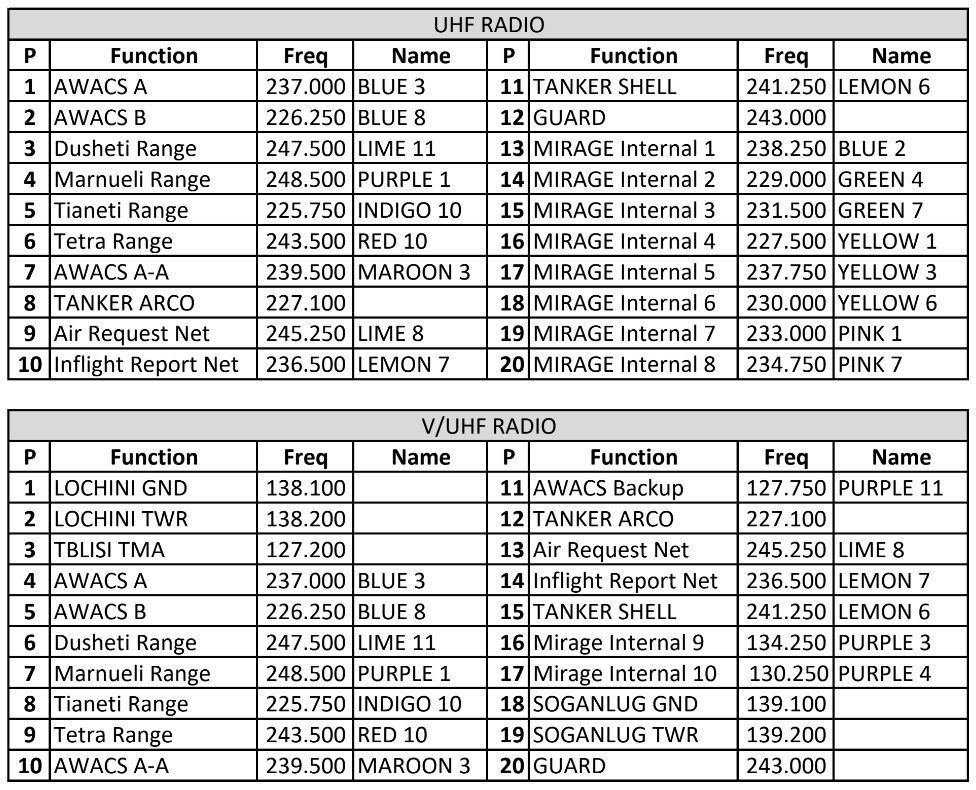
\includegraphics[scale=0.65]{presets.png}
    	\label{presets}
    	\caption{Radio presets for the Mirage 2000C as of January, 2018}
  \end{figure}


\section{Air Tasking Order}
	\textnormal{
    	The 132nd vWing Air Tasking Order (ATO) tasking is based on how actual NATO forces distribute their air taskings and gives a summary of active flights in the upcoming 24h time-period. Reading the ATO is a process called \textit{task fragging}  - hence you will hear the term \textit{as fragged} beeing used during briefs and flights when referring to something being in accordance with the ATO. \\
     }
     
     \textnormal{        
        The ATO has a format suitable for easy transmission over battlefield networks, and as such might seem difficult to decipher at first. However, as a wingman your main concerns should be where you are departing from - and recovering to, as well as your main- and backup internal frequencies. Another important bit of information listed in the ATO is your flights call-sign. The following is an example of an ATO: \\ \\
      \textbf{
      	\footnotesize
          \indent VTASK/132vW/3893/102000ZFEB2015// \\
          \indent TASKUNIT/765th/ICAO:UGTB// \\
          \indent AMSNDAT/TR3893/TR/-/-/54/-/-/DEPLOC:UGTB/ARRLOC:UGTB// \\
          \indent MSNACFT/2/M2000C/FREEDOM31-32/FLIGHT LEAD DISCRETION/ \\
          \indent -/YELLOW9/ORANGE5// \\ \\
      }
    }
    
    \textnormal{
    	From the above the following information can be gathered;
    }
    
    \begin{itemize}
      \item[-] The tasking is for the 132nd vWing, with task number 3893 - and a briefing time of 2000Z
      \item[-] The tasked unit is the 765th, located at UGTB (Tbilisi-Lochini Airport)
      \item[-] Primary mission is mission TR3893, with no secondary mission at this time. Flight is departing from UGTB, and will recover at UGTB as well.
      \item[-] This will be a flight of two Mirage 2000C, call-signs FREEDOM3-1 and FREEDOM3-2, carrying a load-out per flight leads discretion. This means the load-out will be briefed at a later time
      \item[-] The flights primary frequency will be YELLOW9, with ORANGE5 as backup (See figure \ref{opfreqs} for actual frequencies) \\
    \end{itemize}
    

\section{Flight's Comms Chatter}
	\textnormal{
    	After beeing assigned to an event and flight, the TR should make his way to that flights' \textit{Flight Comms Chatter}. This houses the flight-plan information, intentions and any communication necessary in order to perform the assigned task. Most of the information here will be familiar, having looked at the ATO prior, but what is new is the \textit{ENR Intentions}. This is in essence a short-hand flight plan filled in by flight-lead where he makes his intentions for this flight known; How he intends to solve the mission. This is important information for both wingmen and air traffic controllers (ATC/AWACS). Wingmen will need to know what to expect in order to perform better. And air traffic agencies need to know what to expect from this flight in order to provide better services and coordination. \\ \\
        A very straight-forward example could be the following: \\ \\
        \footnotesize
        \textit{DEP WEST \\ AAR (SHELL) \\ RTB via STRAIGHT-IN APP\\ \\}
        \normalsize
        Written out, this means \textit{Flight will depart towards the west, perform air-to-air refueling operations at a tanker with call-sign SHELL - before returning to the air base via a straight-in approach.} The above text is written in short-hand, while still managing to get across the intentions of the flight lead. This is particularly useful for the traffic agencies, as they need to process all intentions from all flights each event. Another example could be: \\ \\
        \footnotesize
        \textit{DEP via MUK \\ AAR AT ARCO \\ BARCAP NORTH: \\ - POSIT: BE 075\degree/80NM/FL280 \\ - CAP: 100\degree/55NM/TACFORM/0.8M \\ RTB via OHB\\ \\}
        \normalsize
        The above should be mostly familiar from the previous example. However, this is a more advanced case - not likely to be seen during TR / IQT training. 
        \footnote{
        	For more information on the terms and brevity used in this example, please refer to your IP or the documents referenced at the beginning of this document
         } 
        This time, the flight is departing via \textit{MUK} - short-hand for MUKHRANI NDB, and will be refueling with tanker, call-sign \textit{ARCO}. The flight will then set up a BARCAP, in this example briefed as \textit{BARCAP NORTH} in the mission documents. Flight lead is then defining the entry-point for this BARCAP, with \textit{POSIT} being brevity for the position of a landmark or a common reference point. In this case \textit{BE} - short-hand for Bullseye. The entry-point is then 75\degree for 80NM from Bulls-eye, and the flight should arrive there at FL280. The following line describes the first leg of the BARCAP from the entry-point; Heading 100\degree for 55NM, in tactical formation at Mach 0.8 \\ \\
    }
   	
  \begin{figure}[!ht]
  	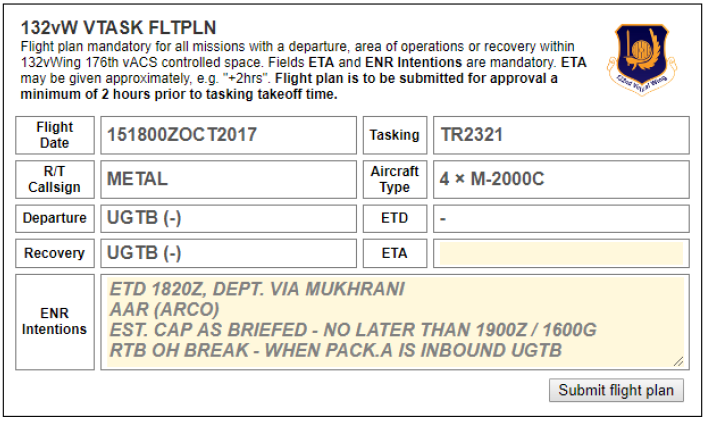
\includegraphics[scale=0.8]{coms-chatter.png}
    	\label{coms-chatter}
    	\caption{Example flight plan from the event-page}
  \end{figure}


\section{After Action Report}
	\textnormal{
    	A proper AAR is very important for both our tactical flying and sharing lessons learned and every participant in an event is expected to submit one. A good AAR and debrief is vital for getting the most out of every event - no matter the out come. In fact, real-life fighter pilots sites the debrief and AAR as the main reason they are able to learn and quickly adapt. Writing the AAR forces the pilot to consciously reflect on certain aspects of the flight that are otherwise easily overlooked. This is especially true if the flight did not go as expected.
    }

\section{TEST}
  \textnormal{
    This is some preview test text. It is very nice indeed!
  }